\documentclass[a4paper, justified]{tufte-handout}

%\geometry{showframe} % display margins for debugging page layout

\usepackage[utf8]{inputenc}
\usepackage{graphicx} % allow embedded images
  \setkeys{Gin}{width=\linewidth,totalheight=\textheight,keepaspectratio}
  \graphicspath{{graphics/}} % set of paths to search for images
\usepackage{amsmath}  % extended mathematics
\usepackage{booktabs} % book-quality tables
\usepackage{units}    % non-stacked fractions and better unit spacing
\usepackage{multicol} % multiple column layout facilities
\usepackage{lipsum}   % filler text
\usepackage{fancyvrb} % extended verbatim environments
  \fvset{fontsize=\normalsize}% default font size for fancy-verbatim environments
\usepackage{multirow} % for table

% Standardize command font styles and environments
\newcommand{\doccmd}[1]{\texttt{\textbackslash#1}}% command name -- adds backslash automatically
\newcommand{\docopt}[1]{\ensuremath{\langle}\textrm{\textit{#1}}\ensuremath{\rangle}}% optional command argument
\newcommand{\docarg}[1]{\textrm{\textit{#1}}}% (required) command argument
\newcommand{\docenv}[1]{\textsf{#1}}% environment name
\newcommand{\docpkg}[1]{\texttt{#1}}% package name
\newcommand{\doccls}[1]{\texttt{#1}}% document class name
\newcommand{\docclsopt}[1]{\texttt{#1}}% document class option name
\newenvironment{docspec}{\begin{quote}\noindent}{\end{quote}}% command specification environment

\title{Report on Tweeter sentiment analysis for Daimler Tech and Data Hub}

\author{Clément Viguier}

\begin{document}

\maketitle% this prints the handout title, author, and date

\begin{fullwidth}
\begin{abstract}
\noindent
This document is a short report on the approaches deployed to take up the Tweeter sentiment analysis challenge. It complements the Jupiter notebook containing the code and provides more insight on the trajectory to solve the problem rather than code explanations.
\end{abstract}

\section{Introduction}
Social media allow new forms of communication, enabling the gathering of people from all around the world with similar centres of interests. While they constitute a formidable opportunity to share ideas and content, they also open the door to uninhibited and toxic interactions. Detecting such messages is a great challenge. Rule-based methods can be used to detect hate speech, but the complexity of the human language combined with the specificity and rapid evolution of short messages on social media make such rules hard to define. Advance computational modelling techniques can help us complement or replace these sets of rules by making sense of extremely large datasets (both in the number of observations and dimensions).

In this report, I document an attempt to build a predictive classification model to identify hateful tweets. Multiple approaches are used, but this is not an exhaustive benchmark of all possible algorithms to approach the problem but rather an overview of my approach to such a problem.

\section{Data integrity and preprocessing}

\subsection{Integrity}

The dataset contains 31,962 tweets, labelled as hateful or not. The dataset is clean, with no apparent empty tweets, or non-labelled values and therefore does not require any strategy to deal with missing values.
However, the data present a high imbalance in the proportion of the type of tweets, with 13 times more non-hateful tweets. This imbalance may put too much focus on the non-hateful tweets, and a balanced sample may be required to improve the prediction of hateful messages.

\subsection{Preprocessing}

The preprocessing of text data consists of clearing the text and preparing the feature construction. In text data, it mostly consists of tokenisation (transform sentences in a group of words) or advances semantic analysis. In the context of tokenisation, the punctuation may contain valuable information (emoticons for example), but it often limits the generalisation of words into features (\textit{word,} is detected as different from \textit{word} creating artificially two feature when one is sufficient). Similarly, the end of words often has a meaning, but it rarely changes the overall idea of its root. Therefore, words can also be group by their root thanks to the stemming process that keeps only the root of words (i.e. \textit{wording} and \textit{words} would both become \textit{word} after stemming), reducing the potential number of feature, while keeping the encapsulated meaning.


\section{The selection of relevant information}

The modelling process for prediction mostly consists of identifying the relevant information. This information is contained in the features of the data and to be relevant this information should:
\begin{enumerate}
\item segregating: allow to distinguish observations in a sample or sub-sample;
\item generalisable: the criterion to segregate observations should be shared (as least partially) with similar observation;
\end{enumerate}
A challenge in machine learning is then to determine which features contain such information, and how the discrimination of the observation should be operated. There is a trade-off here between segregation and generalisation, that translates in modelling terms in a bias-variance trade-off. The choice of the model structure and its hyper-parameters allow adjusting the position of the predictor along this trade-off.

\subsection{The specificity of text data}

\paragraph{Numerous features}

While, at a given time, any language has a finite number of words, these are extremely large and an increasing number of observations goes with an increasing number of features. Similarly, the increasing size of a text observation goes with the increase in its dimensions and its complexity. Moreover, the power of these dimensions can be very dependent on the context, the rarity of a term and its relative frequency in the different classes to predict. The link between the features and the observation has potentially a large impact on the performance of the model.


\paragraph{Unbalanced data}

When sentiment analysis is not used for ranking, it is generally used for the detection of low-frequency behaviour (as the system could not really tolerate high frequencies). This is the case of this problem, leading to a training dataset that contains 13 times more negative observations than positives. This unbalance in observation can lead to fitting problem (a lot of algorithms rely on the global accuracy and is not sensitive to low-frequency classification error), over-fitting (low frequency may lead to generalisation of a few examples) or feature selection (in particular for text data where features depend on the content of the observations).

Finding the good ratio between the number of observations per class in the training dataset might be crucial to have good performances.

\paragraph{Natural language and feature extraction}

Because natural language relies on the diversification of common roots to build words and nuanced meaning, a lot of words differ in their exact spelling (because of conjugation or grammar) but share similar meaning or root idea. Preprocessing steps such as stemming or lemmatising allow to capture this common meaning, or original root, by keeping only the stem of the words observed. The isolation and pruning of words is the base to build a bag of words that represent a sentence and by extension the dimensions of the dataset.

While a bag of word approach allows classifying text, the meaning of a sentence depends also on its structure. Therefore, to refine classifications it may be needed to assess this structure and encode it in new features. This is a particular branch of machine learning that requires both time and expertise. If alternative approaches do not meet the expectations, this direction can be investigated.

\section{Modelling}

With the specificities of the problem in mind, it is time to generate, train and test a classification model to later apply it to the data to train. The choice of the type of model, its hyper-parameters and the (training) sampling strategy will be driven by both the understanding of the data structure and tests.

\subsection{First approach: Naive Bayes}

The Naive Bayes (NB) approach works well for text classification as it the vectorised tokens (frequency of each word) meet the requirements of the features for NB, the algorithm supports a very large number of features and allow classification. The prediction of this approach with little preprocessing (remove mentions and punctuation) will be used as a reference point.

The labelled data is divided between train and test samples with a 70\% - 30\% split.

The training the multinomial NB on the unbalanced sample gives a very good accuracy (0.95\%)(subject to change because of the random sampling) but an average (for a training set) f1-score (0.60) for the training dataset. The test dataset shows similar precision and below average f1-score (0.4).

\paragraph{Sampling}

An unbalanced sampling can cause many problems, here the low f1-score even for the training dataset, is explained by the low number of observation in one-class that lead to a low error rate during the classifier fit. Using a balanced sample with the same classifier greatly improve the f1-score for the training set (0.95) but does not improve the test set score (0.40). 

\begin{table}[]\label{NB1unbalanced}
\begin{center}
\begin{tabular}{llcr}
                                              &                            & \multicolumn{2}{c}{Predicted}                    \\
                                              & \multicolumn{1}{l|}{class} & 0                        & \multicolumn{1}{c}{1} \\ \cline{2-4} 
\multicolumn{1}{c}{\multirow{2}{*}{Observed}} & \multicolumn{1}{c|}{0}     & \multicolumn{1}{r}{8796} & 138                  \\
\multicolumn{1}{c}{}                          & \multicolumn{1}{c|}{1}     & \multicolumn{1}{r}{423  }   & 232                  
\end{tabular}
\caption{Test set confusion matrix of NB model fitted with unbalanced dataset.}
\end{center}
\end{table}

This f1 is due to a large number of false positive. To improve this prediction without changing the type of model: (1) the features can be further cleaned with text processing tools and avoid duplicated features (\textit{i.e.} \texttt{smiles} and \texttt{smile} can be captured by the same feature, see discussion above) and (2) the sampling balance can be improved as an hyper-parameter.

\begin{table}[]\label{NB1balanced}
\begin{center}
\begin{tabular}{llcr}
                                              &                            & \multicolumn{2}{c}{Predicted}                    \\
                                              & \multicolumn{1}{l|}{class} & 0                        & \multicolumn{1}{c}{1} \\ \cline{2-4} 
\multicolumn{1}{c}{\multirow{2}{*}{Observed}} & \multicolumn{1}{c|}{0}     & \multicolumn{1}{r}{7453} & 1481                  \\
\multicolumn{1}{c}{}                          & \multicolumn{1}{c|}{1}     & \multicolumn{1}{r}{56}   & 599                  
\end{tabular}
\caption{Test set confusion matrix of NB model fitted with balanced dataset.}
\end{center}
\end{table}

The stop word removal and stemming decrease the number of features from 52243 to 49183.
In addition, the test on the f1-score as a function of the ratio between the two classes allow to select more informative samples. Samples with 2 to 3 times more negative samples (see figure \ref{ratio} seem to have better performances as they limit the production of false positives (as with an unbalanced sample) while limiting the number of false negatives (even though there is often a trade-off between these two errors for a given level of information).

\begin{figure}\label{ratio}
  \includegraphics[]{images/sample_ratio_TSA.png}
  \caption{Average (n = 10) f1-scores for test datasets as a function of the negative:positive class ratio.}
  \label{fig:marginfig}
\end{figure}

This new training lead to an f1-score of approximatively 0.6555 that is correct. Alternative approaches can be experimented to try to improve this score.

\subsection{Alternative approaches}

\paragraph{Random Forest}

Where a tree can have a strong prediction power but show great over-fitting, Random Forest (RF) have the advantage of this limiting the over-fitting thanks to two mechanisms: (1) feature bootstrapping and (2) the use of multiple small (therefore less prone to over-fitting) trees. However, it is often necessary to optimise the hyper-parameters with cross-validation (CV) procedures, and they tend to be a bit slower. However, the structure of decision trees allow these algorithms and derived (such as RF) to capture easily interactions between features.

When trained with the training test with a ratio negative:positive of 3, this algorithm scores a respectable 0.659 f1-score.

Surprisingly, the hyper-parametrisation does not improve the performance of the random forest. The range of parameter tested could be adjusted (see table \ref{RF-HP} for details). However, because such exploration of parameter space is computationally expensive, experimentation of other algorithms is preferred here.

\begin{table}[]\label{RF-HP}
\begin{tabular}{l|ccccc}
Hyper-parameter & \multicolumn{5}{l}{Values}                                  \\ \hline
n\_estimators   & 10             & 20      & \textbf{100*} & 200         & 500 \\
max\_features   & \textbf{0.3*}  & auto    & log2          &             &     \\
max\_depth      & 5              & 6       & 7             & \textbf{8*} &     \\
criterion       & \textbf{gini*} & entropy &               &             &     \\ 
\end{tabular}
\caption{Hyperparameters for random forest algorithm. The \textbf{bold*} values mark the result of the optimisation by a 3 fold cross-validation procedure.}
\end{table}


\paragraph{Feature selection}

The mutual information criterion allows reducing the number of features by ranking them based on the relationship between the variables to explain. This, however, leads to a disappointing score (0.48). These results suggest that the work should not necessarily be on the selection of features. This could be explained by the intuition that contrarily to many machine learning problem, the information is not hidden in complex relationships between features (even though words may change meaning depending on the context) but rather the information is diffused within large feature sets.

Extracting new (or additional) feature may help improve the prediction. 

%\paragraph{Adaboost}
\paragraph{New features and lexicons}

New features can be extracted from the text by considering the punctuation and other structural features. Lexicon, that links common words with emotions (8 basic emotions or negative and positive) can also be used to add information. Indeed, because these lexicons (that are results of the classification model themselves) are based on large dataset external to the training set, they provide more information.

For the current problem, the features are not merged to the original features. Both modelling (by RF, data not shown, f1-score around 0.3) and visualising (see figure \ref{sentiment}) the relationship between these features and the variable to predict show only week correlations (small effect of joy and anger sentiments). While these lexicons open new trajectories, the work (and RAM) needed to explore them without certainty on the result pushes toward other directions.

\begin{figure}\label{sentiment}
  \includegraphics[]{images/sentiment_scores.png}
  \caption{Pairplot of the sentiment score of tweets in the balanced sample for 4 emotions out of 8.}
\end{figure}

It seems more valuable to spend more time trying to understand where the classification error come from to address this specific problem, and not rely on the assumption that additional information (new features or new observations) is needed.


\subsection{Understanding the error}

\paragraph{Shifting error}

Shifting from an unbalanced sample (negative:positive = 13) to more balanced one (negative:positive = 3) leads to a shift from false negative error to false positive, with the same features. This suggests a shift in the weight of each feature toward a particular class. This can be investigated by plotting the link between the feature and the two classes (\texttt{hateful} or \texttt{non-hateful}). This score is estimated by computing the relative proportion of a term in the hateful tweet class. A term, or token, that appears in 4 hateful tweets and 1 non-hateful tweet will have a \textit{hatefulness} score of 80\%. This method is used to score all feature and visualise them.


The large majority of words have null or low scores (see figure \ref{hatefulness}, explained by the high number of non-hateful tweets. While it makes sense that there are more words with a non-hateful score if there are more non-hateful tweets, this unbalance may bias this score. Indeed, if we imagine a frequently used term with a neutral meaning (neither hateful or non-hateful), it would have a strong relationship with the most common class. 

\begin{figure}\label{hatefulness}
  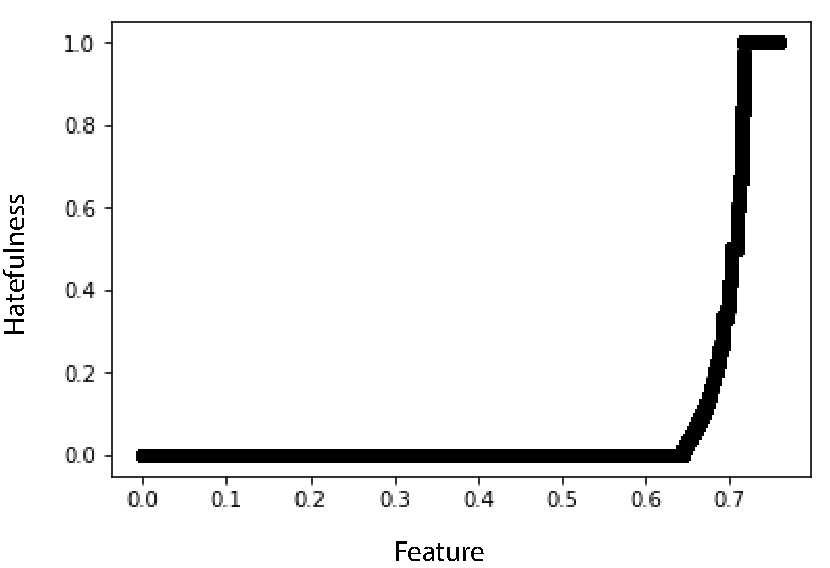
\includegraphics[]{images/hatefulness.pdf}
  \caption{Hatefulness (0: non-hateful, 1: hateful) scores of all features in the training set.}
  \label{fig:marginfig}
\end{figure}

With the intuition that the distribution of observation may change the relative perception of a term, we can understand how the sampling affects the type of error. While a model fitted on unbalanced data will classify a large number of false negatives (see table \ref{NB1unbalanced}) if the negative are numerous (resulting in numerous features biased toward this class), the same type of model fitted with a balanced dataset will predict much more positives (and false positives, see table \ref{NB1balanced}). This is explained by the shift toward more hateful scores has the number of non-hateful observation decreases (see figure \ref{hatefulness_corrected}, showing an important shift of most features). On one hand, this resampling increases the f1-score by balancing the class and limit the false-negative by correcting the hatefulness of some features. On the other hand, the reduction of samples also leads to the reduction of meaningful features (a lot of features are not represented, especially non-hateful features) leading to a high number of false-positives. There is a trade-off that limits the progress that can be made by manipulating the samples alone.

\begin{figure}\label{hatefulness_corrected}
  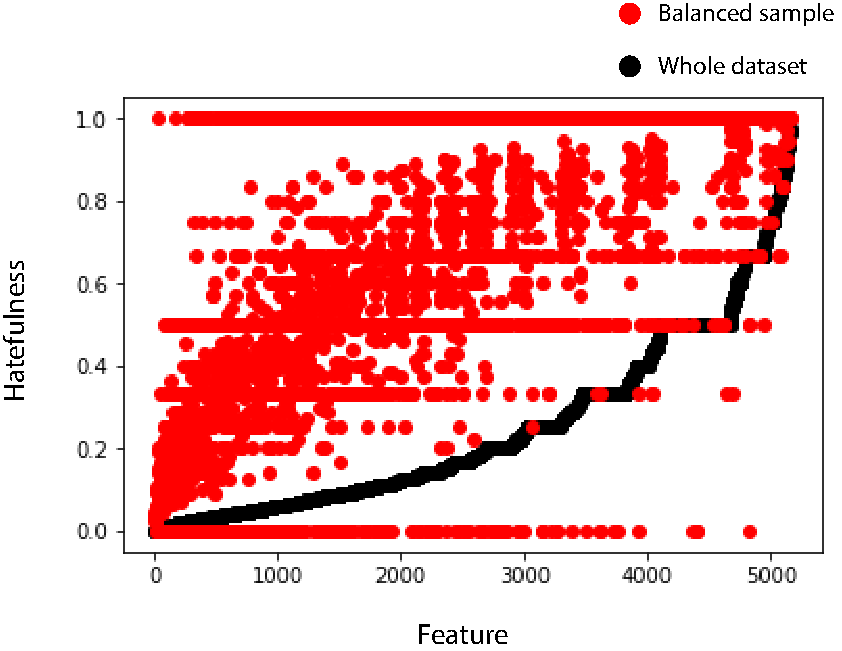
\includegraphics[]{images/hatefulness_corrected.pdf}
  \caption{Hatefulness (0: non-hateful, 1: hateful) scores of ambiguous features ($0 < hatefulness < 1$). Black dots mark the hatefulness computed for the whole dataset, the red dots represent the hatefulness of the same features computed with a balanced dataset (negative:positive = 1). All points above the dark point-line are feature that had their hatefulness under-estimated due to the unbalance  distribution.}
  \label{fig:marginfig}
\end{figure}



\textit{(The hatefulness is not really used by the model presented in this report, but it illustrates the relationship between the explaining and explained variables and helps to understand the relationship between this relationship captured by the models and the sample balance.\\
The hatefulness of words may be used to compute a composite feature for the tweet like the average hatefulness of a tweet. This feature could be used by algorithms that do not support a large amount of features (tens of thousands of features are used here). In this case, this metric should be corrected by the proportion of observations in each class.)}

\subsection{Constructing a hybrid approach}

NB and RF can handle numerous variables but are sensitive to sampling because of the relative information phenomenon illustrated in the previous section. However, with a smart model design, the illustrated trade-off can be partly untied. Indeed, the use of two successive classifiers with two different samples allows reducing the error by artificially changing the strength of the feature as a function of the type of tweet. Unbalanced samples lead to a polarised error that can be negated by a second round of classification. The idea is to use the strength of a model to classify the observations that are non ambiguous, and let another model deal with the ambiguous observations (\textit{i.e.} the observation predicted of the class with the most errors, for example, the observation predicted as negative when there is a lot of false negatives). The second model is then trained with a model better to classify these observations. To obtain the second model, you use all the observations predicted as ambiguous (of the class with the most errors, in this example negatives) to fit the model. Because of this filtering, the fitting process focuses on ambiguous tweets and reduce one type of error, while limiting the impact on the second type of error.

\begin{table}[]\label{final}
\begin{center}
\begin{tabular}{llcr}
                                              &                            & \multicolumn{2}{c}{Predicted}                    \\
                                              & \multicolumn{1}{l|}{class} & 0                        & \multicolumn{1}{c}{1} \\ \cline{2-4} 
\multicolumn{1}{c}{\multirow{2}{*}{Observed}} & \multicolumn{1}{c|}{0}     & \multicolumn{1}{r}{8891} & 18                  \\
\multicolumn{1}{c}{}                          & \multicolumn{1}{c|}{1}     & \multicolumn{1}{r}{371  }   & 309                  
\end{tabular}
\caption{Test set confusion matrix of the two rounds model (NB + RF) fitted with unbalanced dataset then ambiguous dataset.}
\end{center}
\end{table}

This two-step model, by focussing on difficult cases allow a better predict. There is still a risk of over-fitting illustrated by the good fit to the train data (f1 = 0.89 for the model illustrated in table \ref{final}) that is not reproduced with the test date (f1 = 613). The test result for the best model cannot be presented as the whole dataset was used to train it.

Hyper-parameter search and additional steps may be needed to get better f1-scores. The use of lexicon to deal with the ambiguous observation may also improve the classification.


\section{Conclusion}

The work-flow to answer the classification problem of hateful tweets lead to the production of a predictive model with a reasonable f1-score (0.705). While this score can certainly be improved, the process of building this model also gave insight on the role of the samples on the information given by the features.

More advanced techniques (such as neural networks) that require optimisation of hyper-parameters and that can handle complex interactions between predictors could be explored to further improve the predictive performance of the model. In the context of natural language, the semantic analysis that integrate the nature of words and their links are certainly the next step to produce a high-performance model without long and computationally expensive parameter space explorations and deep learning algorithms. While a first idea to explore is the association of negative words that change the sense of a feature, more complex analysis can consider the grammatical role of a word (noun, verb, adverb, adjective, etc...) to get closer to a human understanding of the phrase structure and therefore a better prediction.

\newpage
\begin{table*}\label{scores}
\begin{tabular}{l|ccc|cc|cc}
Approach:                                                        & \multicolumn{3}{c|}{Naive Bayes}   & \multicolumn{2}{c|}{Random Forest} & \multicolumn{2}{c}{Hybrid} \\
Details:                                                         & no cleaning & lemmatising & MI    & 100 est.         & Opti. CV        & NB + RF      & RF + RF      \\ \hline
f1-score                                 & 0.529        & .655        & 0.483 & 0.659            & 0.435           & 0.615        & 0.701       \\
ratio neg:pos & 13           & 3           & 3     & 3                & 3               & 13       & 13     \\
   
\end{tabular}
\vspace{1cm}
\caption{Summary table of f1-scores and sample properties of the approaches tested. The sampling neg:pos ratio is the relative ratio between the number of observations in each class. The hybrid approach uses two different samples (that overlap) to fit the two classifiers. All model but the first where fitted with lemmatised data. Notation: NB: Naive Bayes, RF: Random Forest, CV: cross-validation, MI: mutual Information criteria, est.: estimators, opti.: optimised by grid search. }
\end{table*}


\bibliography{daimler}
\bibliographystyle{plainnat}


\end{fullwidth}


\end{document}
